\section{ANEXOS TÉCNICOS}

\subsection{Anexo A: Definición del Esquema DDL en Neon PostgreSQL (schema.sql)}
A continuación se presenta un extracto fundamental del esquema relacional DDL implementado en Neon Serverless PostgreSQL, destacando el catálogo maestro, la partición mensual de series de tiempo y las funciones disparadoras reactivas desacopladas.

\begin{lstlisting}[language=SQL, caption={Extracto DDL de Tablas y Triggers Desacoplados en schema.sql}]
-- 1. Catalogo Maestro Inmutable de SKUs
CREATE TABLE IF NOT EXISTS catalogo_productos_master (
    sku_id VARCHAR(255) PRIMARY KEY,
    producto VARCHAR(255) NOT NULL,
    cadena VARCHAR(100) NOT NULL,
    departamento VARCHAR(100) NOT NULL,
    sucursal VARCHAR(100),
    categoria VARCHAR(100),
    laboratorio VARCHAR(100),
    presentacion VARCHAR(255),
    unidad_medida VARCHAR(50),
    enlace_canonico TEXT,
    imagen TEXT,
    created_at TIMESTAMP WITH TIME ZONE DEFAULT CURRENT_TIMESTAMP,
    updated_at TIMESTAMP WITH TIME ZONE DEFAULT CURRENT_TIMESTAMP
);

-- 2. Historico de Precios Particionado Mensualmente
CREATE TABLE IF NOT EXISTS precios_historico (
    id BIGSERIAL,
    fecha DATE NOT NULL,
    sku_id VARCHAR(255) NOT NULL,
    precio_actual_bs NUMERIC(10, 2) NOT NULL,
    precio_anterior_bs NUMERIC(10, 2),
    descuento_pct NUMERIC(5, 2),
    delta_precio_bs NUMERIC(10, 2),
    delta_porcentaje NUMERIC(6, 2),
    disponible BOOLEAN DEFAULT TRUE,
    recorded_at TIMESTAMP WITH TIME ZONE DEFAULT CURRENT_TIMESTAMP,
    PRIMARY KEY (sku_id, fecha)
) PARTITION BY RANGE (fecha);

-- Particion Mensual para Noviembre 2026
CREATE TABLE IF NOT EXISTS precios_historico_2026_11 
    PARTITION OF precios_historico
    FOR VALUES FROM ('2026-11-01') TO ('2026-12-01');

-- 3. Funcion Reactiva Desacoplada para Medicamentos
CREATE OR REPLACE FUNCTION fn_replicate_medicamento_to_master()
RETURNS TRIGGER AS $$
DECLARE
    v_sku VARCHAR(255);
    v_prev_price NUMERIC(10, 2);
    v_delta_bs NUMERIC(10, 2) := NULL;
    v_delta_pct NUMERIC(6, 2) := NULL;
BEGIN
    v_sku := 'MED_' || UPPER(REGEXP_REPLACE(NEW.cadena, '\s+', '_', 'g')) || '_' ||
             UPPER(REGEXP_REPLACE(NEW.producto, '[^a-zA-Z0-9]+', '_', 'g'));

    INSERT INTO catalogo_productos_master (
        sku_id, producto, cadena, departamento, categoria, 
        laboratorio, presentacion, enlace_canonico, imagen
    ) VALUES (
        v_sku, NEW.producto, NEW.cadena, NEW.departamento, NEW.categoria,
        NEW.laboratorio, NEW.presentacion, NEW.enlace, NEW.imagen
    )
    ON CONFLICT (sku_id) DO UPDATE SET
        enlace_canonico = COALESCE(EXCLUDED.enlace_canonico, catalogo_productos_master.enlace_canonico),
        imagen = COALESCE(EXCLUDED.imagen, catalogo_productos_master.imagen),
        updated_at = CURRENT_TIMESTAMP;

    -- Calculo de Variacion respecto al registro inmediatamente anterior
    SELECT precio_actual_bs INTO v_prev_price
    FROM precios_historico
    WHERE sku_id = v_sku AND fecha < NEW.fecha
    ORDER BY fecha DESC LIMIT 1;

    IF v_prev_price IS NOT NULL AND v_prev_price > 0 THEN
        v_delta_bs := ROUND(NEW.precio_bs - v_prev_price, 2);
        v_delta_pct := ROUND(((NEW.precio_bs - v_prev_price) / v_prev_price) * 100, 2);
    END IF;

    INSERT INTO precios_historico (
        sku_id, fecha, precio_actual_bs, precio_anterior_bs, descuento_pct,
        delta_precio_bs, delta_porcentaje, disponible
    ) VALUES (
        v_sku, NEW.fecha, NEW.precio_bs, NEW.precio_anterior_bs, NEW.descuento_pct,
        v_delta_bs, v_delta_pct, NEW.disponible
    )
    ON CONFLICT (sku_id, fecha) DO UPDATE SET
        precio_actual_bs = EXCLUDED.precio_actual_bs,
        precio_anterior_bs = EXCLUDED.precio_anterior_bs,
        descuento_pct = EXCLUDED.descuento_pct,
        delta_precio_bs = EXCLUDED.delta_precio_bs,
        delta_porcentaje = EXCLUDED.delta_porcentaje,
        disponible = EXCLUDED.disponible;

    RETURN NEW;
END;
$$ LANGUAGE plpgsql;
\end{lstlisting}

\subsection{Anexo B: Procedimiento de Backfill In-Engine (backfill.sql)}
El script de backfill reconstruye de manera retrospectiva el catálogo maestro y los deltas de variación histórica a partir de las tablas operacionales preexistentes:

\begin{lstlisting}[language=SQL, caption={Procedimiento de Migracion y Calculo de Deltas en backfill.sql}]
-- Replicacion masiva controlada de observaciones operacionales
INSERT INTO catalogo_productos_master (
    sku_id, producto, cadena, departamento, sucursal, categoria, enlace_canonico, imagen
)
SELECT DISTINCT ON ('CANASTA_' || UPPER(REGEXP_REPLACE(fuente, '\s+', '_', 'g')) || '_' || UPPER(REGEXP_REPLACE(producto, '[^a-zA-Z0-9]+', '_', 'g')))
    'CANASTA_' || UPPER(REGEXP_REPLACE(fuente, '\s+', '_', 'g')) || '_' || UPPER(REGEXP_REPLACE(producto, '[^a-zA-Z0-9]+', '_', 'g')),
    producto, fuente, departamento, fuente, categoria, enlace, imagen
FROM canasta_precios
ORDER BY 'CANASTA_' || UPPER(REGEXP_REPLACE(fuente, '\s+', '_', 'g')) || '_' || UPPER(REGEXP_REPLACE(producto, '[^a-zA-Z0-9]+', '_', 'g')), fecha DESC
ON CONFLICT (sku_id) DO NOTHING;
\end{lstlisting}

\clearpage
\subsection{Anexo C: Catálogo Técnico de Selectores DOM Validados}
En la Tabla~\ref{tab:anexo_selectores} se detallan los selectores CSS y patrones de extracción validados en los scrapers de Playwright.

\begin{table}[htbp]
    \centering
    \small
    \caption{Catálogo Técnico de Selectores DOM e Indicadores Dinámicos en Scrapers}
    \label{tab:anexo_selectores}
    \begin{tabularx}{\linewidth}{>{\raggedright\arraybackslash}p{3.3cm} >{\raggedright\arraybackslash}p{4.2cm} L}
        \toprule
        \textbf{Plataforma} & \textbf{Elemento Objetivo} & \textbf{Selector DOM / Expresión Regular} \\
        \midrule
        Hipermaxi & Contenedor de Producto & \nolinkurl{div.product-item}, \nolinkurl{div.card-product} \\
        Hipermaxi & Título y Marca & \nolinkurl{h3.product-title}, \nolinkurl{.brand-name} \\
        Hipermaxi & Precio Unitario & \nolinkurl{.product-price}, \nolinkurl{span.price-value} \\
        Hipermaxi & Flag Scroll Infinito & \texttt{span:has-text("Obteniendo más productos")} \\
        Farmacorp & Tarjeta de Producto & \nolinkurl{.product-item}, \nolinkurl{.grid-item} \\
        Farmacorp & Paginador Numérico & \nolinkurl{nav.pagination}, \nolinkurl{.pagination__item} \\
        Farmacorp & Precio y Descuento & \nolinkurl{.price--highlight}, \nolinkurl{.price--compare} \\
        Farmacias Chávez & Paginación Simple & \nolinkurl{.ant-pagination-simple-pager} (\texttt{/\textbackslash s*(\textbackslash d+)/}) \\
        Farmacias Chávez & Selector de Tarjeta & \nolinkurl{div[class*="ProductCard"]}, \nolinkurl{.ant-card} \\
        Farmacias Chávez & Botón Siguiente Página & \nolinkurl{.ant-pagination-next:not(.ant-pagination-disabled)} \\
        \bottomrule
    \end{tabularx}
    \tablenote{Resumen de los selectores DOM optimizados en el código fuente de los scrapers.}
\end{table}

\clearpage
\subsection{Anexo D: Plataformas Web de Comercio Retail y Farmacéutico Auditadas}
Para documentar la fisonomía y complejidad visual de las fuentes de datos analizadas, la Figura~\ref{fig:tiendas_retail_storefronts} presenta las interfaces de usuario de las cadenas farmacéuticas inspeccionadas.

\begin{figure}[htbp]
    \centering
    \caption{Portales Web Comerciales de Farmacorp y Farmacias Chávez}
    \label{fig:tiendas_retail_storefronts}
    \begin{minipage}{0.49\linewidth}
        \centering
        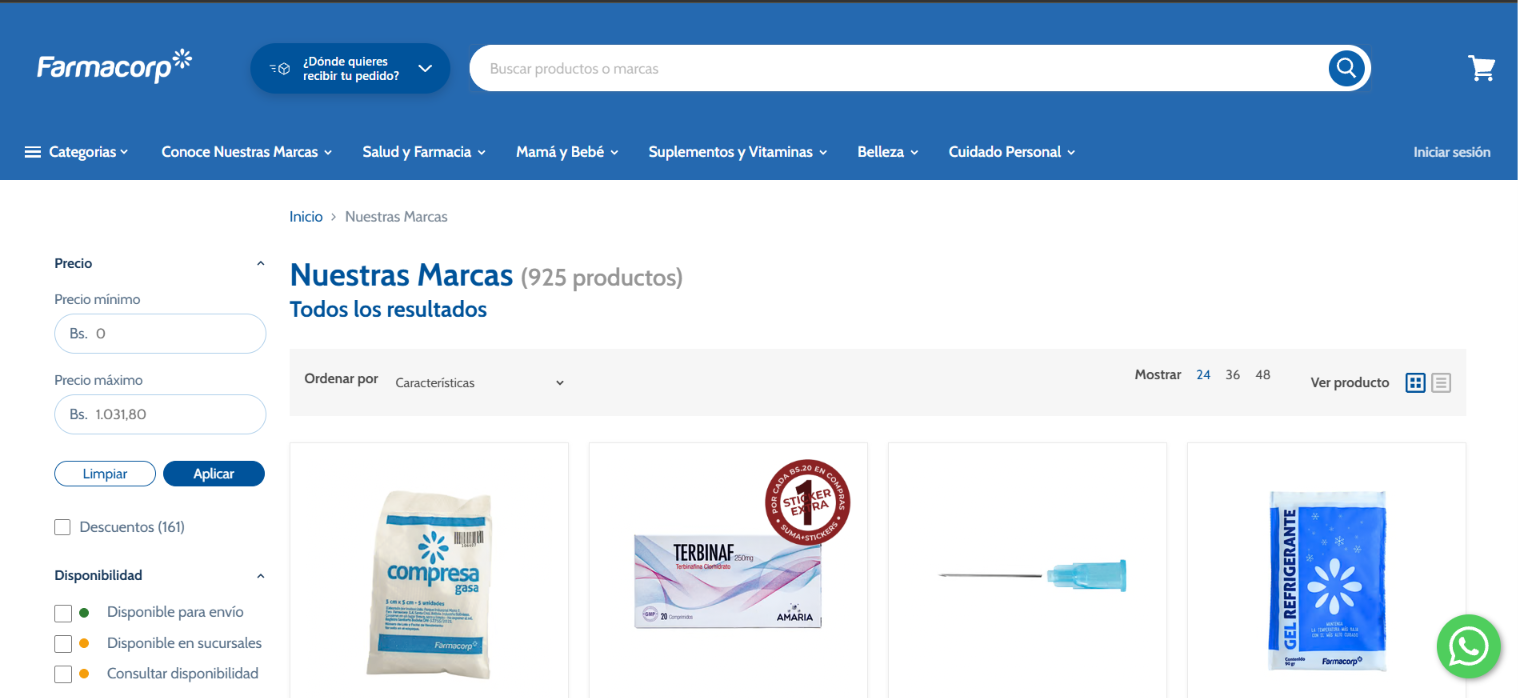
\includegraphics[width=\linewidth]{figuras/imgFarmacorpStore.png}
        \caption*{(a) Tienda digital Farmacorp (Shopify)}
    \end{minipage}\hfill
    \begin{minipage}{0.49\linewidth}
        \centering
        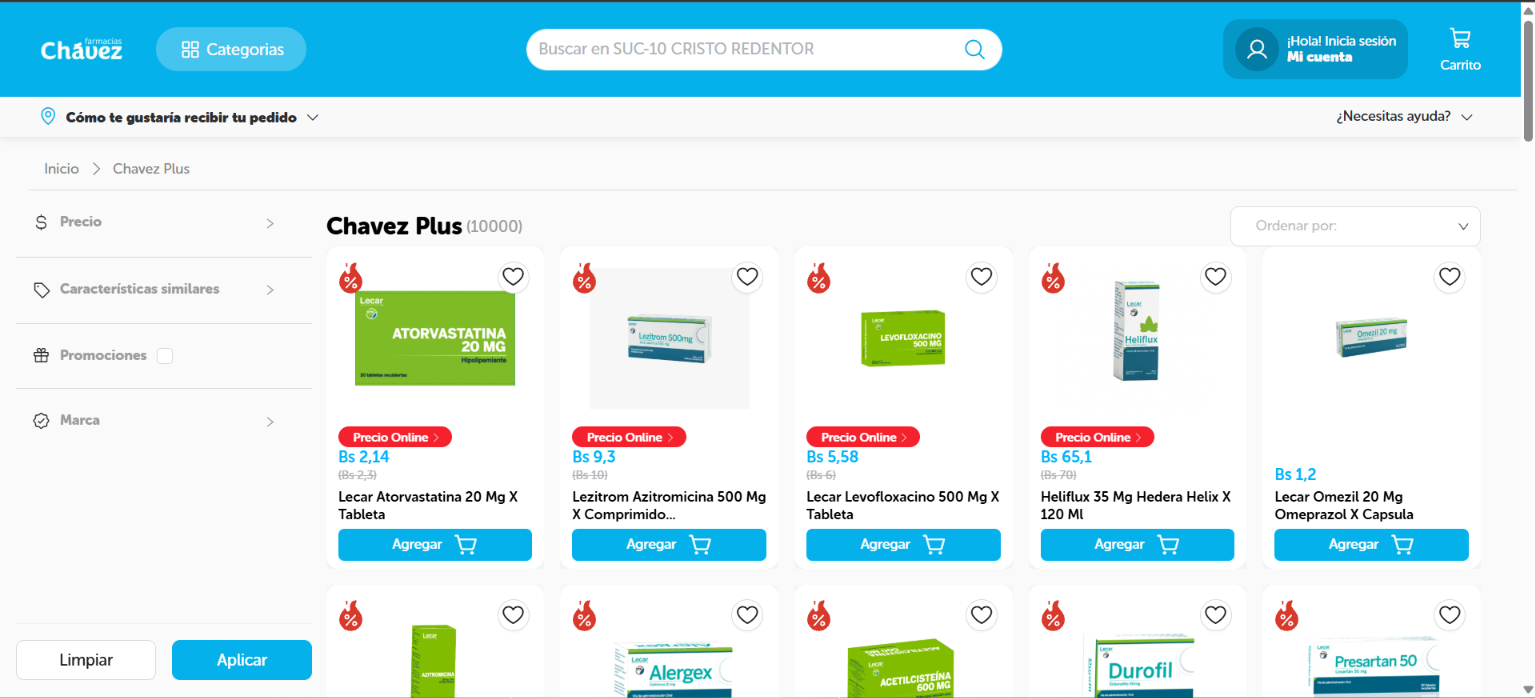
\includegraphics[width=\linewidth]{figuras/imgChavezStore.png}
        \caption*{(b) Tienda digital Farmacias Chávez (Next.js)}
    \end{minipage}
    \figurenote{Capturas de los portales comerciales de comercio electrónico de Farmacorp y Farmacias Chávez, evidenciando las estructuras de catálogo, banners promocionales y filtros facetados analizados por los scrapers.}
\end{figure}
